\documentclass[12pt,a4paper]{article}
\usepackage[utf8]{inputenc}
\usepackage[T1]{fontenc}
\usepackage[french]{babel}
\usepackage{lmodern,microtype}
\usepackage[margin=2.5cm]{geometry}
\usepackage{graphicx}
\graphicspath{{images/}}
\usepackage{booktabs}
\usepackage{tabularx}
\usepackage{array}
\usepackage[table]{xcolor}
\usepackage{enumitem}
\usepackage{amsmath}
\usepackage{calc}      
\usepackage{float}
\usepackage{siunitx}
\sisetup{locale=FR}
\usepackage{needspace}
\usepackage{pdfpages}
\usepackage{tikz}
\usetikzlibrary{arrows.meta,positioning}
\usepackage{csquotes}
\usepackage{longtable}
\usepackage{array}
\usepackage{siunitx} 
\usepackage[backend=biber,style=numeric,sorting=none]{biblatex}
\addbibresource{refs.bib}
\usepackage[hidelinks]{hyperref} % Load last

\definecolor{rvert}{RGB}{198,239,206}
\definecolor{rjaune}{RGB}{255,235,156}
\definecolor{rrouge}{RGB}{255,199,206}

% Column types used in tables
\newcolumntype{Y}{>{\raggedright\arraybackslash}X}
\newcolumntype{P}[1]{>{\raggedright\arraybackslash}p{#1}}

% TikZ diagram styles
\tikzset{
  block/.style={draw,align=center,text width=43mm,minimum height=12mm,inner sep=3pt,font=\small,line width=0.4pt},
  arrow/.style={-{Latex[length=2mm]},line width=0.5pt}
}

% Marker for items to be completed
\newcommand{\todo}[1]{\textcolor{orange}{\textit{[To be completed: #1]}}}
\newcommand{\mot}[1]{\textbf{#1}}

\title{SIMPLEX ARGUS Project: MCR Report}
\author{Adnane AIT ZIDANE, Taha EL OUALI, Ahmadou SALL, \\
Thomas WEBER, Brian YOUMBI DIESSE}
\date{Updated on \today}

\begin{document}
\maketitle
\tableofcontents
\newpage

% =====================================================================
\section{General Project Information}

\begin{tabularx}{\textwidth}{@{}>{\bfseries}p{5cm}Y@{}}
\toprule
Last updated & 7 October 2026 \\
Programme & M2 Newspace \\
Team / project name & DeOrbit (ARGUS project) \\
Project coordinators & Adnane Ait Zidane and Thomas Weber \\
Coordinators' email addresses & adnaneaitzidane@outlook.com -- thweber@outlook.fr \\
\bottomrule
\end{tabularx}

% =====================================================================
\section{Project Overview}


The ARGUS project aims to detect a piece of space debris and then modify its
trajectory using a laser, with the entire system hosted on a 6U nanosatellite.
The concept rests on three interdependent elements: the \textbf{design} of the debris and the satelite, 
\textbf{debris detection},\textbf{laser-induced trajectory modification},and its complete instrument suite.

This is an experimental project: a satellite of this size cannot generate high
power levels. It nevertheless provides a means of testing the feasibility of
modifying the trajectory of debris using a space-based laser. The velocity
changes achievable with this technology would be of the order of metres per
second. Figure~\ref{fig:chrono} shows the mission timeline.

\begin{figure}[h]
  \centering
  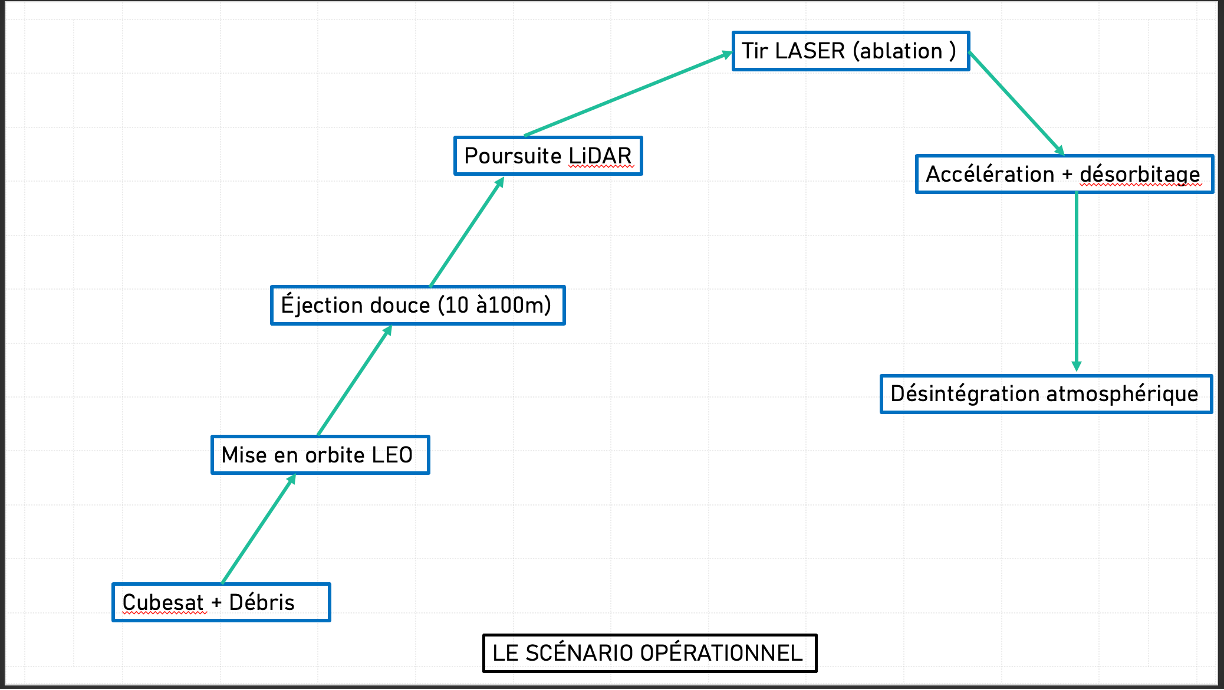
\includegraphics[width=0.8\textwidth]{chrono_argus.png}
  \caption{ARGUS mission timeline}
  \label{fig:chrono}
\end{figure}

{
  \small
  \setlength{\parindent}{0pt}
  \setlength{\parskip}{5pt}
  \renewcommand{\arraystretch}{1.15}
  \setlength{\tabcolsep}{5pt}
  % ============================================================
% risk_matrix.tex : include with \input{risk_matrix.tex}
% (does NOT contain \begin{document})
%
% Packages required in the main preamble:
%   \usepackage{booktabs}
%   \usepackage{longtable}
%   \usepackage{array}
%   \usepackage{amsmath}
%   \usepackage{xcolor}
% ============================================================

\subsubsection*{9.1 Mission 5$\times$5 Risk Matrix}\label{mission-55-risk-matrix}

% --- 5x5 matrix ---------------------------------------------
\begin{table}[htbp]
\centering
\small
\setlength{\tabcolsep}{4pt}
\renewcommand{\arraystretch}{1.3}
\begin{tabular}{
  >{\centering\arraybackslash}p{2.6cm}
  *{5}{>{\centering\arraybackslash}p{2.1cm}}
}
\toprule
\textbf{Likelihood $\backslash$ Consequence} & \textbf{1 (Negligible)} & \textbf{2 (Minor)} & \textbf{3 (Moderate)} & \textbf{4 (Critical)} & \textbf{5 (Catastrophic)} \\
\midrule
\textbf{5 (Very High)} & --- & --- & --- & --- & --- \\
\textbf{4 (High)}      & --- & \textbf{R-03} & --- & --- & --- \\
\textbf{3 (Moderate)}  & --- & \textbf{R-05} & \textbf{R-04} & --- & --- \\
\textbf{2 (Low)}       & --- & --- & \textbf{R-01} & \textbf{R-02} & --- \\
\textbf{1 (Very Low)}  & --- & --- & --- & --- & --- \\
\bottomrule
\end{tabular}
\end{table}

% --- Risk register ------------------------------------
{\small
\setlength{\tabcolsep}{3pt}
\renewcommand{\arraystretch}{1.2}
\begin{longtable}{@{}
  >{\raggedright\arraybackslash}p{0.08\linewidth}
  >{\raggedright\arraybackslash}p{0.27\linewidth}
  >{\centering\arraybackslash}p{0.04\linewidth}
  >{\centering\arraybackslash}p{0.04\linewidth}
  >{\raggedright\arraybackslash}p{0.35\linewidth}
  >{\raggedright\arraybackslash}p{0.12\linewidth}@{}}
\toprule
\textbf{Risk ID} & \textbf{Risk Title \& Description} & \textbf{L} & \textbf{C} & \textbf{Mitigation Strategy} & \textbf{Owner} \\
\midrule
\endfirsthead
\toprule
\textbf{Risk ID} & \textbf{Risk Title \& Description} & \textbf{L} & \textbf{C} & \textbf{Mitigation Strategy} & \textbf{Owner} \\
\midrule
\endhead
\bottomrule
\endfoot
\bottomrule
\endlastfoot

\textbf{R-01} & \textbf{EPM Release Stiction:} Residual flux or mechanical stiction prevents target release. & 2 & 3 & Dual-wound coil with 200\% reverse demagnetization current; Delrin guide pins; TVAC bakeout testing. & Mechanisms Lead \\

\textbf{R-02} & \textbf{Premature Target Release:} Launch vibration separates target from dispenser. & 2 & 4 & Magnetic retention force rated $>18\text{ N}$ ($>100\text{ g}$ holding); mechanical retaining lips block lateral shear. & Structures Lead \\

\textbf{R-03} & \textbf{Solar Storm Rapid Reentry:} Elevated solar flux ($F_{10.7} > 220$) reduces orbit life to $<30\text{ days}$. & 4 & 2 & 350 km baseline provides 3.5-month margin; expedited CONOPS executes laser firing within 18 days of launch. & Mission Design Lead \\

\textbf{R-04} & \textbf{Target Tracking Dropout:} Tumbling coupon causes optical tracking fades at standoff. & 3 & 3 & Primary tracking utilizes onboard lidar and micro-CCR; 2 cm sphere carried as active challenger. & GNC Lead \\

\textbf{R-05} & \textbf{Optics Plume Contamination:} Ablated plume deposits material on beam director primary mirror. & 3 & 2 & Standoff maintained at $300$--$500\text{ m}$; plume expansion density falls off as $1/R^2$, dropping to zero deposition beyond $10\text{ m}$. & Payload Lead \\

\end{longtable}
}
}

\section{Project Feasibility}
{
  \small
  \setlength{\parindent}{0pt}
  \setlength{\parskip}{5pt}
  \renewcommand{\arraystretch}{1.15}
  \setlength{\tabcolsep}{5pt}
  
This section assesses the feasibility of the ARGUS mission. 
To do so, we need to calculate certain key parameters essential to successful mission execution. 
These calculations should also validate our various parameter choices, 
particularly those relating to the selected LASER sources, 
the debris material and the target orbit.  
\subsection{Theoretical Calculation of Selected LASER Parameters}
\begin{itemize}
    \item \textbf{Ablation Threshold and Optimal Fluence (F)}\\
    The fluence of our LASER at a wavelength of $\lambda = 1064 nm$ with pulses of \textbf{nanosecond duration (ns)} 
    represents the energy deposited by this laser per unit area. It is expressed in \textbf{$J/cm^{2}$}. 
    The scientific literature places the theoretical ablation threshold between $F_{th} \approx 1 J/cm^{2}$ and $F_{th} \approx 2   J/cm^{2}$ (Philippe class reference).
    However, to obtain the required optimal propulsive effect in our case, we need to reach the maximum coupling fluence $F_{couplage}$ defined by: \\
    \begin{equation}
    \boxed{F_{couplage} \approx  2.5 F_{th} \approx  5 J/cm^{2}}
    \end{equation}
    for $F_{th} = 2 J/cm^{2}$\\

    \item \textbf{Pulse energy \textbf{$E_{P}$} and peak power \textbf{$P_{c}$}}\\
    Pulse energy represents the total energy contained in a single LASER pulse. 
    It is calculated using the following formula: 
    \begin{equation}
        \boxed{E_{P} = S *  F_{couplage} }
    \end{equation}
    $S$ represents the area illuminated by the LASER pulse. 
    For a selected focal spot diameter of $d = 0.3 cm$ and assuming a spherical spot, we obtain the value of $S$ :  
    \begin{equation}
      \boxed{  S = \frac{\pi d^{2}}{4} =\frac{\pi * (0.3)^{2}}{4} \approx 0.071 cm^{2} }
    \end{equation}
    With this value of $S$, we finally obtain: 
    \begin{equation}
        \boxed{E_{P} = 0.071 *5 = 0.35J }
    \end{equation}
    Thus, with this value of $E_{P}$, we can determine the instantaneous peak power \textbf{$P_{c}$} generated by our LASER. This power represents the energy flow per unit time. It is the maximum power reached by the LASER within the pulse itself. It is obtained by dividing the pulse energy by the pulse duration. 
    \begin{equation}
        \boxed{P_{c} = \frac{E_{P}}{\tau} = \frac{0.35}{5.10^{-9}} = 70MW}
    \end{equation}
    \\
    \item \textbf{Repetition rate $f_{rep}$ and average power $P_{moy}$}\\
    To accommodate the payload within a $6U$ CubeSat, we assume an average power of $P_{moy} = 1000 W$. 
    This value is not arbitrary; it is primarily dictated by the thermal dissipation limit of a $6U$ CubeSat \cite{Bekey1997,Phipps2012}.\\
    With this value, the pulse repetition rate is calculated using the formula below: \\
    \begin{equation}
        \boxed{f_{rep} = \frac{P_{moy}}{E_{P}} = \frac{1000W}{0.35 J}  = 2857 Hz \approx 3KHz}
    \end{equation}
    
\end{itemize}

\subsection{Calculation of $\Delta V$ and Deorbiting Dynamics}
The calculation of the required velocity change $\Delta V$ and the transferred impulse is based on three main elements: \\
\begin{itemize}
    \item \textbf{The momentum coupling coefficient ($C_{m}$)}\\
    When a LASER beam interacts with the surface of a material at a fluence above its ablation threshold (aluminium in this case),
    the material vaporises instantaneously. This ejection of matter, the \textbf{rocket effect}, generates a recoil force. 
    This coefficient measures the efficiency with which the LASER transfers momentum to the debris. The coupling is defined by the following fundamental relationship \cite{Phipps2012}:\\
    \begin{equation}
        \boxed{C_{m} = \frac{I}{E_{LASER}} = \frac{\Delta p}{E_{LASER}}}
    \end{equation}
    with \textbf{I} the total generated impulse (\textbf{$N.S$}) and \textbf{$E_{LASER}$} the total absorbed LASER energy in (\textbf{J}). $C_{m}$ is expressed in (\textbf{$N.s/J$}).\\
    According to the experimental data in \cite{Phipps2012} for a nanosecond LASER at a wavelength of $\lambda = 1064nm$, the stabilised value at peak fluence is equal to $C_{m} = 30 \mu N.s/J$\\

    \item \textbf{Average generated force $F_{moy}$}\\
    This force is therefore given by the expression below:
    \begin{equation}
       \boxed{ F_{moy} = c_{m} * P_{moy} = 30.10^{-6} * 1000 = 0.03N = 3 mN}
    \end{equation}\\

    \item \textbf{Orbital dynamics }\\
    In our case, we opt for a staged atmospheric re-entry, lowering the debris perigee and allowing the atmosphere to complete the process. We therefore apply our LASER impulse directly opposite to the velocity vector \textbf{$\vec{v_{debris}}$} of the debris at apogee.\\
    According to the vis-viva equation and Kepler's laws, we define the circular velocity \textbf{$\vec{{v_{c}}}$} of the debris in its initial orbit (at \textbf{$350 Km$} ).
    This is the velocity required for the centrifugal force to balance Earth's gravity exactly and maintain its trajectory.
    \begin{equation}
       \boxed{ {v_{c}} = \sqrt{\frac{\mu}{R_{E} + h}} = \sqrt{\frac{3.986.10^{14}}{6371000 + 350000}} = 7701 m/s }
    \end{equation}

To lower its perigee to a critical altitude of \textbf{$h_{p}= 100Km$}, the velocity at the new apogee \textbf{$\vec {v_{a}}$} is given by: 
\begin{equation}
  \boxed{  v_{a} = \sqrt {\mu \left(\frac{2}{r_{a}} -\frac{2}{r_{a} + r_{P}}\right )} = \sqrt {3.986.10^{14}\left(\frac{2}{6371000 + 350000} -\frac{2}{6721000 + 6471000}\right )} = 7628 m/s}
\end{equation}
Here, $r_{a} = R_{E} + h$, represents the apogee radius of the new trajectory;\\
$r_{P} = R_{E} + h_{P}$, represents the perigee radius of the new trajectory.\\
We select a LEO orbit at $h = 350Km$, which is the initial orbit of our debris (corresponding to the initial orbit of our CubeSat).\\
$h_{P} = 100Km$ corresponds to the target altitude of the debris. At this orbit, the atmosphere is sufficiently dense to decelerate our debris and cause re-entry. \\
$\mu = 3.986.10^{14} m^{3}/s^{2}$ is Earth's standard gravitational parameter.\\
$R_{E} \approx 6371 Km$ represents Earth's mean radius.\\
The expression for $\Delta V$ is therefore written as follows: 
\begin{equation}
    \boxed{\Delta V = v_{c} - v_{a} = 7701 -7628 = 73m/s}
\end{equation}
Numerical result: $\boxed{\Delta V = 73  m/s}$.\\
The total required firing duration can also be calculated. \\
\begin{equation}
    \boxed{\Delta t = \frac{m_{debris} * \Delta V}{F_{moy}} = \frac{1* 73}{0.03} = 2433 s }
\end{equation}
The required firing duration $\Delta t $ is approximately $40$ minutes and $33$ seconds to impart a velocity change of $\Delta V = 73$ $m/s$ to our debris,
divert it from its initial orbit and cause atmospheric re-entry. \cite{Vallado2013}\\

But it's impossible to keep the contact between the debris and the CubeSat for 40 minutes.
It's no nessecary to create a big $\Delta V$ if you change the orbit with a small $\Delta V$ and wait for the debris to re-enter the atmosphere it's a success.
Thanks to this experimental project, we will be able to validate the feasibility of our concept and the effectiveness of our LASER ablation system in space.

\end{itemize}

}

\section{Design and Debris Management}


The shapes of both the nanosatellite and the debris must be selected. The shape
of the debris has a major influence on atmospheric re-entry. The means of
providing the required power (batteries and solar panels) and managing overheating
must be selected according to mission requirements.

\begin{itemize}
  \item \textbf{Nanosatellite geometry}: the structure is designed around a 6U
  format. The dimensions under consideration are $30 \times 20 \times 10$~cm
  or $60 \times 10 \times 10$~cm, although other configurations remain possible.
\end{itemize}

The two next parts of the report describe the LiDAR and laser systems, and the machine learning algorithms used for debris detection and tracking.
The both part is the main instrumentation of the nanosatellite, and the most critical for the success of the mission.

\section{LiDAR and Laser}
{
  \small
  \setlength{\parindent}{0pt}
  \setlength{\parskip}{5pt}
  \renewcommand{\arraystretch}{1.15}
  \setlength{\tabcolsep}{5pt}
  % ---------- Payload ----------

Sizing a LASER-ablation deorbiting system involves a direct physical trade-off:
 the LASER must not destroy the debris through excessive heat input, 
 but must vaporise a very thin layer of its surface to create a propulsive plasma that slows the moving debris. 
 Thus, modifying the orbit of an object (debris) relies on converting the optical energy deposited by laser pulses into the mechanical energy of the plasma jet.

\subsection{LASER Ablation Propulsion}
When a high-intensity LASER beam strikes the surface of a material, 
the optical energy is absorbed instantaneously. 
The temperature of the surface layer rises so rapidly that it undergoes sudden sublimation and becomes a highly energetic plasma. 
This jet of matter is expelled at very high speeds. Under the physical law of conservation of matter, the ejection of matter generates a mechanical recoil force on the target object \cite{Vincent2011}.

\begin{figure}[H]
  \centering
  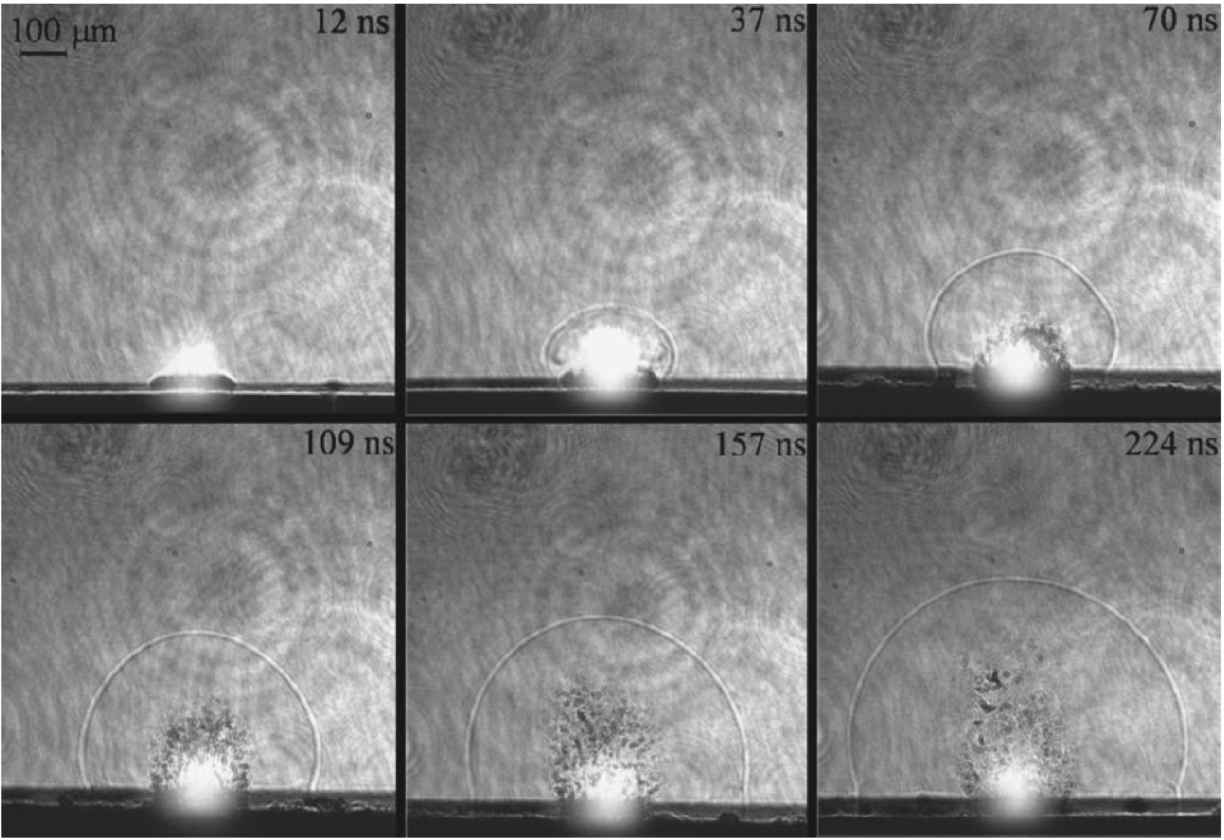
\includegraphics[width=0.8\textwidth,height=7cm,keepaspectratio]{ablation_laser.png}
  \caption{Images of the ablation propulsion process at different times during the laser--aluminium interaction for $\lambda = 1064 nm$ and $\tau = 5ns$. The propagation of the shock wave over time can be observed. \cite{Vincent2011}}
  \label{fig:ablation}
\end{figure}

\subsection{High-Power LASER Characteristics}
In this section, we describe the characteristics of our onboard high-power LASER. 
Selecting the high-power LASER is crucial: if its power or energy is unsuitable, 
it will probably not be possible to initiate the micropropulsion process at the surface of our target (debris).

\begin{enumerate}
    \item \textbf{Choice of LASER type:}\\
    We choose a pulsed LASER rather than a continuous-wave laser. 
    The factors determining this choice are summarised in the table below

    \begin{table}[H]
      \centering
      \caption{Comparison between continuous-wave and pulsed lasers.}
      \begin{tabular}{p{3.5cm} p{5.5cm} p{5.5cm}}
        \toprule
        \textbf{Characteristic} & \textbf{Continuous-wave laser } & \textbf{Pulsed laser} \\
        \midrule
        Effect on debris & Thermal melting  & Plasma ablation (mechanical rocket effect) \\
        Peak power & Equal to average power  & Several megawatts during the pulse \\
        Generated thrust & Almost zero at this power level & Optimal and directional \\
        Risks & High risk of breaking up the debris & Safe, targeted surface action \\
        \bottomrule
      \end{tabular}
    \end{table}

    \item \textbf{Required LASER parameters:}\\
    The wavelength of our high-power LASER is set to $\lambda = $\SI{1064}{\nano\metre} in the infrared, with a pulse duration of \textbf{nanoseconds (ns)}. This choice is primarily based on the absorption characteristics of the material making up our debris, namely aluminium (Al).

    For this CubeSat project using a $6U$ platform firing a LASER at short range, the optimal average power required for our small aluminium debris object, measuring \SIrange{1}{10}{\centi\metre} and weighing $1kg$ is approximately $1000W$. The choice of this operating power is deliberate and results from a specific trade-off validated by orbital mechanics and the physics of laser--matter interaction. The section on project feasibility discusses in detail the importance of reaching this optimal LASER ablation power.

    \begin{table}[H]
      \centering
      \small
      \caption{Ablation laser parameters.}
      \label{tab:laser_ablation}
      \begin{tabular}{p{6cm} p{6cm}}
        \toprule
        \textbf{Parameter} & \textbf{Value} \\
        \midrule
        Wavelength ($\lambda$) & \SI{1064}{\nano\metre} (infrared) \\
        Operating mode & Pulsed \\
        Pulse duration ($\tau$) & Nanosecond (ns) \\
        Average power ($P_{\text{moy}}$) & \SI{1000}{\watt} (\SI{1}{\kilo\watt}) \\
        Repetition rate ($f$) & \SI{3000}{\hertz} (\SI{2}{\kilo\hertz}) \\
        Pulse energy ($E_p$) & \SI{0.5}{\joule} \\
        Peak power ($P_{\text{crête}}$) & \SI{100}{\mega\watt} \\
        Ablation threshold fluence & \SIrange{1}{2}{\joule\per\centi\metre\squared} \\
        Optimal coupling fluence & \SI{5}{\joule\per\centi\metre\squared} \\
        \bottomrule
      \end{tabular}
    \end{table}
\end{enumerate}

\subsection{LiDAR for Detection}
To meet the imposed dimensional constraints, we favour a micro-LiDAR over a conventional LiDAR, which would entail higher mass and energy demands. The micro-LiDAR provides optical metrology of the debris: detection, relative position and relative velocity \cite{OpromollaNocerino}. It consists of three main elements:
\begin{itemize}
    \item The emission source, which in our case could be a VCSEL (Vertical Cavity Surface Emitting LASER). These are arrays of miniature semiconductor LASERs. The table below summarises the parameters we consider optimal for defining the LASER source of our micro-LiDAR.

    \begin{table}[H]
      \centering
      \small
      \caption{Micro-LiDAR laser parameters \cite{VCSEL1550_2023}.}
      \label{tab:lidar_laser}
      \begin{tabular}{p{3.3cm} p{4.7cm} p{6.5cm}}
        \toprule
        \textbf{Parameter} & \textbf{Specified value} & \textbf{Purpose in space} \\
        \midrule
        Wavelength & \SI{1550}{\nano\metre} & Prevents blinding by the ablation laser (\SI{1064}{\nano\metre}) \\
        Source type & Pulsed laser diode (InGaAs) & Robustness, extreme compactness \\
        Pulse duration & \SI{3}{\nano\second} & Millimetre-level ranging accuracy \\
        Frequency & \SI{20}{\kilo\hertz} & Smooth real-time target tracking \\
        Pulse energy & \SI{10}{\micro\joule} & Completely harmless to the debris \\
        Electrical power consumption & $\approx\SI{12}{\watt}$ & Fully suited to the constraints of a 6U CubeSat \\
        \bottomrule
      \end{tabular}
    \end{table}

    \item An ultrasensitive SPAD (Single Photon Avalanche Diode) detector. These detectors can detect a single returning photon. The table below summarises the parameters we consider optimal for selecting a suitable detector for our micro-LiDAR \cite{Pellegrini2006}.

    \begin{table}[H]
      \centering
      \small
      \caption{Micro-LiDAR SPAD detector parameters \cite{SPADReview2024}.}
      \label{tab:lidar_spad}
      \begin{tabular}{p{3.3cm} p{4.7cm} p{6.5cm}}
        \toprule
        \textbf{Parameter} & \textbf{Specified value} & \textbf{Purpose in space} \\
        \midrule
        Detector type & SPAD InGaAs/InP & Sensitive at \SI{1550}{\nano\metre}, single-photon detection \\ % to be verified
        Detection efficiency & $\approx\SI{20}{\percent}$ at \SI{1550}{\nano\metre} & Detect the weak signal backscattered by the debris \\ % to be verified
        Timing jitter (\textit{jitter}) & $\approx\SI{200}{\pico\second}$ & Range resolution of a few centimetres \\ % to be verified
        Dark count rate & $\approx\SI{10}{\kilo\hertz}$ (cooled detector) & Limit noise to maintain a good signal-to-noise ratio \\ % to be verified
        Operating mode & Gated (\textit{gated}), synchronised with the pulse & Reduce noise and power consumption \\ % to be verified
        \bottomrule
      \end{tabular}
    \end{table}

    \item MEMS (Micro-Electro-Mecanical System) micromirrors. These oscillating micromirrors are etched into silicon to steer the beam without heavy mechanical components. The table below summarises the parameters we consider optimal for selecting the mirror assembly for our micro-LiDAR \cite{Shea2006}.

    \begin{table}[H]
      \centering
      \small
      \caption{Micro-LiDAR oscillating MEMS micromirror parameters \cite{Liu2022}.}
      \label{tab:lidar_mems}
      \begin{tabular}{p{3.3cm} p{4.7cm} p{6.5cm}}
        \toprule
        \textbf{Parameter} & \textbf{Specified value} & \textbf{Purpose in space} \\
        \midrule
        Scanning mechanism & Resonant MEMS micromirror & Scene scanning without bulky mechanical components \\ % to be verified
        Mirror diameter & $\approx\SI{1}{\milli\metre}$ & Trade-off between optical aperture and resonant frequency \\ % to be verified
        Optical scan angle & $\pm\SI{10}{\degree}$ & Cover the field of view required for target acquisition \\ % to be verified
        Resonant frequency & $\approx\SI{1}{\kilo\hertz}$ & Scan rate compatible with real-time tracking \\ % to be verified
        Electrical power consumption & Less than $\SI{1}{\watt}$ & Compatible with the power budget of a 6U CubeSat \\ % to be verified
        \bottomrule
      \end{tabular}
    \end{table}
\end{itemize}


}

\section{Machine Learning and Intelligent Debris Detection}

{
  \small
  \setlength{\parindent}{0pt}
  \setlength{\parskip}{5pt}
  \renewcommand{\arraystretch}{1.15}
  \setlength{\tabcolsep}{5pt}
  \subsection{Vision Pipeline Organisation}
The vision system estimates the \textbf{position and orientation of the debris}, 
then tracks its relative motion. It combines Auricam images, 
two neural networks and a geometric calculation based on camera calibration and a metrically scaled 3D model of the debris.

\begin{center}
\begin{tikzpicture}[node distance=8mm and 7mm]
\node[block] (cam) {\textbf{Auricam D35}\\Monochrome image};
\node[block,right=of cam] (ssd) {\textbf{SSD-MobileNetV2}\\Debris bounding box};
\node[block,right=of ssd] (hr) {\textbf{HRNet-W32}\\Image keypoints};
\node[block,below=of hr] (pnp) {\textbf{SQPnP}\\Position and orientation};
\node[block,left=of pnp] (ukf) {\textbf{Adaptive UKF}\\Tracking and uncertainty};
\node[block,left=of ukf] (out) {\textbf{Time-stamped result}\\Pose and motion};
\draw[arrow](cam)--(ssd);
\draw[arrow](ssd)--(hr);
\draw[arrow](hr)--(pnp);
\draw[arrow](pnp)--(ukf);
\draw[arrow](ukf)--(out);
\end{tikzpicture}
\end{center}
{\small Initialisation sequence. During tracking, the UKF uses the observed keypoints and predicts the region of interest in the next image.}

The target rate is two optical observations per second, processed as they are acquired. The detector runs at initialisation, during full-image checks and after tracking is lost. 
Between these calls, the predicted region allows processing to focus on the debris.

\subsection{Camera: Monochrome Auricam D35, 25 mm Focal Length}
We select the optical head \textbf{Sodern Auricam D35}, including its baffle,
 to capture the outline and geometric features of the debris. Monochrome imaging avoids colour demosaicing;
 the global shutter exposes all pixels simultaneously~\cite{sodern_auricam}.

\begin{tabularx}{\linewidth}{|P{36mm}|Y|}
\hline
\textbf{Characteristic} & \textbf{Configuration and published specifications}\\\hline
Sensor & $2048\times2048$ pixels; pixel pitch of $5{,}5\,\mu\mathrm{m}$; global shutter.\\\hline
Optics & 25 mm focal length; standard aperture $f/3{,}5$; field of view of $35^\circ$ diagonally, approximately $25^\circ$ along each side.\\\hline
Frame rate & Full frame, 12-bit: 2,5 frames/s. Binning $2\times2$: 10 frames/s at $1024\times1024$.\\\hline
Interface & SpaceWire, up to 160 Mbit/s.\\\hline
Power supply & 4,6--6 V; published power consumption of 2 W.\\\hline
Integration & $80\times80\times140$ mm including baffle; mass of 420 g.\\\hline
\end{tabularx}

The 25 mm focal length combines a useful image scale with a framing margin. 
A projected dimension of 30 cm at 10 m spans approximately 136 native pixels. 
The optics and mounting are calibrated, and the focus is then adjusted for the observation range of 2 to 10 m. 
Pointing complies with the published Sun exclusion angle of $38^\circ$.

\subsection{Onboard Computing: Q8S, XE2 and Interfaces}
The \textbf{Xiphos Q8S} receives the images, prepares the network inputs and runs SQPnP, 
the UKF and data logging. The \textbf{CogniSAT-XE2} from Ubotica runs the neural networks on its Myriad X processor~\cite{xiphos_q8s,ubotica_xe2}.

\begin{tabularx}{\linewidth}{|P{29mm}|Y|Y|}
\hline
\textbf{Equipment} & \textbf{Key specifications} & \textbf{Role in Argus}\\\hline
Xiphos Q8S & Zynq UltraScale+ XCZU7EG ; 4 Cortex-A53, 2 Cortex-R5 and FPGA ; 4 GB of error-correcting RAM; 5 W typical. & Reception, cropping, data preparation, pose estimation and temporal tracking.\\\hline
CogniSAT-XE2 & Myriad X ; PC/104 form factor; 80 g typical; 2,5 W typical with a representative network and Ethernet. & Execution of SSD-MobileNetV2 and HRNet-W32; return of results to the Q8S.\\\hline
Carrier board & Power supplies, connectors and interface circuits. & Camera connection and integration of the SpaceWire interface with the Q8S FPGA.\\\hline
\end{tabularx}

Images arrive via SpaceWire; the Q8S communicates with the XE2 over Ethernet. Integration verifies the camera data rate, the ARM64 Linux host software and the loading of both networks. Tests measure the latency between exposure and output, as well as the power consumption of the complete system.

The vision system coste around 22 W, including margins and conversion losses, with an allocation of 1 kg and 2U covering the camera, boards and interfaces. These design allocations are separate from the typical power consumption of the equipment.

\subsection{Neural Networks: Detection Followed by Keypoint Localisation}
\textbf{SSD-MobileNetV2} receives an image prepared at $320\times320$ pixels. It searches for the debris and returns a bounding box with a score. This architecture is documented for onboard spacecraft pose estimation~\cite{black2021pose}. The bounding box selects the region to be analysed.

\textbf{HRNet-W32} receives this region, extracted from the original image and resized to $256\times256$ pixels. It locates the keypoints associated with the 3D model: corners, junctions or asymmetric features~\cite{fanizza2023pose}. The Q8S maps their coordinates back to the native image; SQPnP initialises the pose, and the UKF then performs tracking.

The networks are trained on the ground using synthetic and real images of the debris under varied lighting conditions. The detector also receives images without debris. Onboard, the weights remain fixed and the models run in FP16. Validation on the XE2 checks keypoint accuracy after compilation, false detections and the processing rate of the complete pipeline.


}

% 


% =====================================================================
\section{Project Management Tools}

\begin{tabularx}{\textwidth}{@{}>{\bfseries}p{5cm}Y@{}}
\toprule
Storage (Drive) & Asana(Notion) / Google Drive \\
Communication & WhatsApp / Google Meet \\
Task tracking & Asana(JIRA) \\
Scheduling & Asana(JIRA) / Instagantt(JIRA) \\
Report preparation & LaTeX \\
\bottomrule
\end{tabularx}

% =====================================================================
\section{Project Organisation}

\subsection{WBS}

\begin{figure}[htbp]
  \centering
  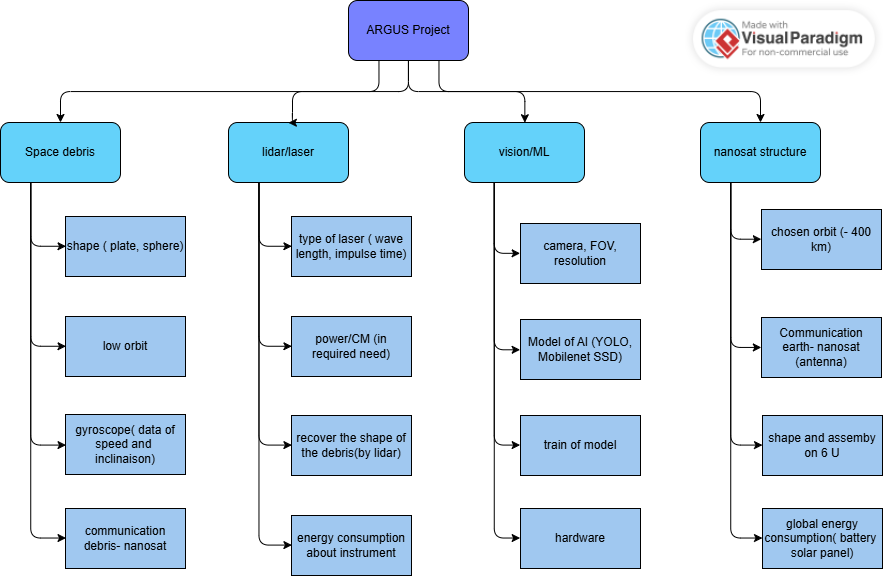
\includegraphics[width=\textwidth]{WBS.png}
  \caption{Project WBS}
\end{figure}

\subsection{Roles and Allocated Resources}

\begin{center}
\begin{tabular}{lll}
\toprule
\textbf{Name} & \textbf{Role} & \textbf{Time allocation} \\
\midrule
Adnane AIT ZIDANE & Coordinator and Structure Team Lead & 5h/week \\
Taha EL OUALI & Vision and Machine Learning Team Lead & 7h/week \\
Ahmadou SALL & LiDAR and Laser Team Lead & 5h/week \\
Thomas WEBER & Coordinator and Systems Engineer & 7h/week \\
Brian YOUMBI DIESSE & Systems Engineer & 5h/week \\
\bottomrule
\end{tabular}
\end{center}

\subsection{Backward Scheduling}

\textit{Status: in progress.}
An issue with our Asana account means that the entire schedule must be recreated
on another platform: \textbf{JIRA}



\subsection{List of Experts}

\begin{tabularx}{\textwidth}{@{}lY@{}}
\toprule
\textbf{Identified experts} & \textbf{Area of expertise} \\
\midrule
Ahmadou Sall, Phillipe KECKHUT & LiDAR and laser systems\\
TBC & orbit \\
Charlotte Corbelle & Project management\\
\bottomrule
\end{tabularx}

\subsection{Risk Analysis}


{\small
\setlength{\tabcolsep}{3pt}
\renewcommand{\arraystretch}{1.2}
\begin{longtable}{@{}
  >{\raggedright\arraybackslash}p{0.07\linewidth}
  >{\raggedright\arraybackslash}p{0.30\linewidth}
  >{\centering\arraybackslash}p{0.04\linewidth}
  >{\centering\arraybackslash}p{0.04\linewidth}
  >{\centering\arraybackslash}p{0.06\linewidth}
  >{\raggedright\arraybackslash}p{0.37\linewidth}@{}}
\toprule
\textbf{ID} & \textbf{Risk} & \textbf{P} & \textbf{S} & \textbf{Crit.} & \textbf{Mitigation} \\
\midrule
\endfirsthead
\toprule
\textbf{ID} & \textbf{Risk} & \textbf{P} & \textbf{S} & \textbf{Crit.} & \textbf{Mitigation} \\
\midrule
\endhead
\bottomrule
\endfoot
\bottomrule
\endlastfoot
 
\textbf{R1} & Poor communication between subteams & 3 & 5 & 15 & Fixed weekly meeting, written minutes, designated contact for each interface \\
\textbf{R2} & Mass, power or volume budgets exceeded & 3 & 4 & 12 & Maintain an up-to-date budget table; review at each milestone \\
\textbf{R3} & Schedule delays and uneven workload distribution & 4 & 3 & 12 & Backward scheduling in Asana, milestones and a 20 \% contingency \\
\textbf{R4} & Temporary unavailability of a team member & 4 & 2 & 8 & Assign a backup for each task; share documentation \\
\textbf{R5} & Dependence on a single expert & 2 & 4 & 8 & Summary notes and external experts \\
\textbf{R6} & Lost or disorganised documents & 3 & 2 & 6 & Single repository, naming conventions and backups \\
\textbf{R7} & Asana issue & 5 & 2 & 10 & Find an alternative (Notion) \\
\end{longtable}
}
 
\vspace{1em}
\begin{table}[htbp]
\centering
\small
\setlength{\tabcolsep}{4pt}
\renewcommand{\arraystretch}{1.8}
\begin{tabular}{
  >{\centering\arraybackslash}p{2.0cm}
  *{5}{>{\centering\arraybackslash}p{1.7cm}}
}
 & \multicolumn{5}{c}{\textbf{Severity}} \\
\cmidrule(lr){2-6}
\textbf{Prob.} & \textbf{1} & \textbf{2} & \textbf{3} & \textbf{4} & \textbf{5} \\
\midrule
\textbf{1} & \cellcolor{rvert} & \cellcolor{rvert} & \cellcolor{rvert} & \cellcolor{rvert} & \cellcolor{rvert} \\
\textbf{2} & \cellcolor{rvert} & \cellcolor{rvert} & \cellcolor{rvert} & \cellcolor{rjaune}\textbf{R5} & \cellcolor{rjaune}\textbf{R7} \\
\textbf{3} & \cellcolor{rvert} & \cellcolor{rvert}\textbf{R6} & \cellcolor{rjaune} & \cellcolor{rjaune}\textbf{R2} & \cellcolor{rrouge}\textbf{R1} \\
\textbf{4} & \cellcolor{rvert} & \cellcolor{rjaune}\textbf{R4} & \cellcolor{rjaune}\textbf{R3} & \cellcolor{rrouge} & \cellcolor{rrouge} \\
\textbf{5} & \cellcolor{rvert} & \cellcolor{rjaune} & \cellcolor{rrouge} & \cellcolor{rrouge} & \cellcolor{rrouge} \\
\bottomrule
\end{tabular}
\end{table}
 
\newpage
% =====================================================================
\section{Team MIRO Board}

\begin{figure}[h]
  \centering
  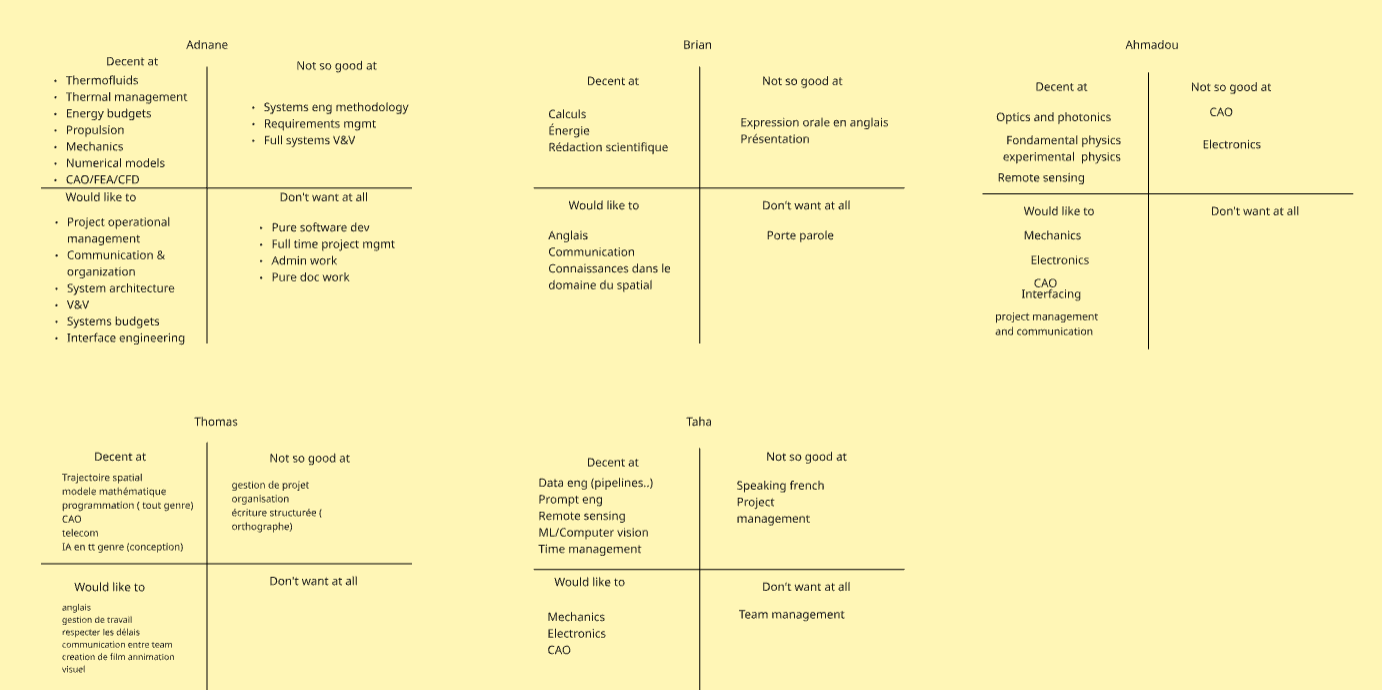
\includegraphics[width=\textwidth]{miro.png}
  \caption{Team MIRO Board}
\end{figure}
% =====================================================================

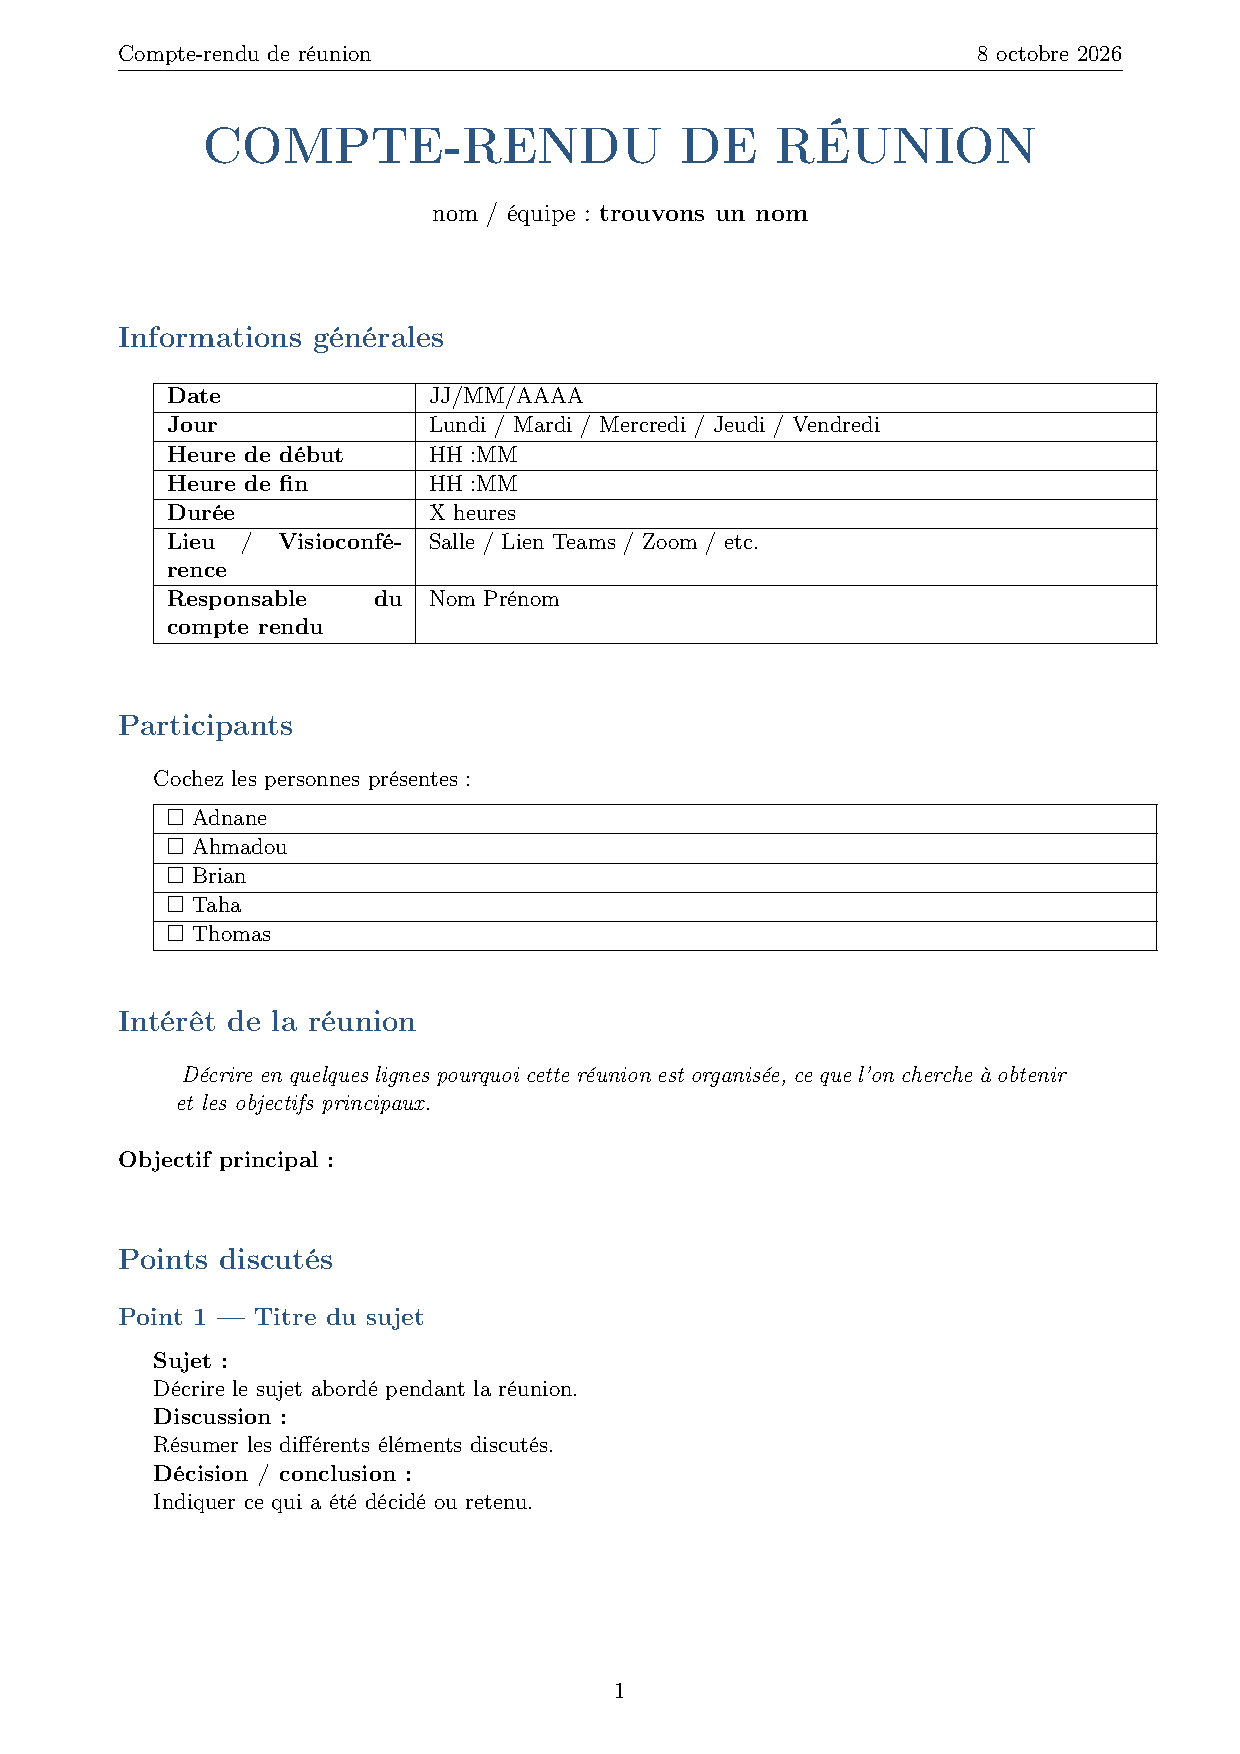
\includepdf[pages=-]{template_réunion.pdf}

\printbibliography[title={References}]
\end{document}